\section{Theoretical Analysis}
\label{sec:analysis}
In this section, the RC circuit shown in Figure~\ref{fig:circuit} is analysed
theoretically. We will begin by analyzing the circuit by applying the nodal method to determine the voltages in all nodes and currents in all branches for t\textless 0.

In order to do this laboratory, we will not only use the node method, but also apply the Thévenin/Norton Theorem as well as what was lectured about capacitors.
%A resistor-capacit circuit (RC circuit) is an electric circuit composed by resistors and capacitors.
A RC circuit is composed by resistors and capacitors and it may driven by voltage or current sources wich will produce different responses.
A capacitor is an electrical component that behaves according to the following differential equations:
\begin{equation}
  q(t)=C\cdot v(t)\Leftrightarrow \frac{d\cdot v(t)}{dt} = C\cdot \frac{d\cdot q(t)}{dt}\Leftrightarrow i(t)=C\cdot \frac{d\cdot v(t)}{dt}
\end{equation}

Thereafter, the current of a capacitor is not proportional to the voltage in its terminals, but rather to the voltage variation rate.

\subsection{Voltages in Nodes and Currents in Branches}

\begin{figure}[H] \centering
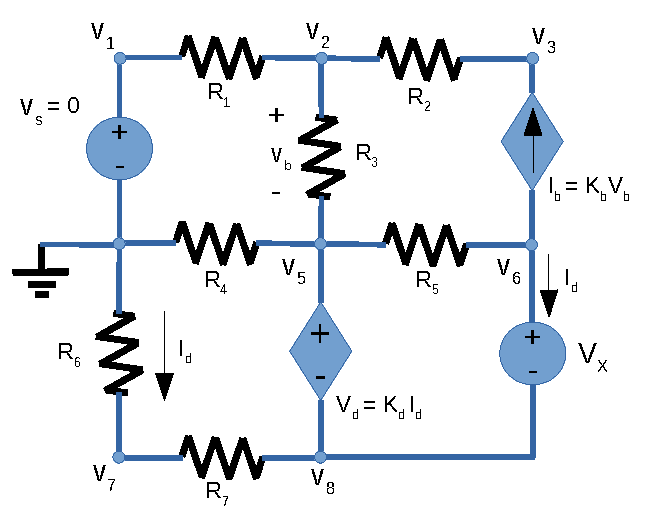
\includegraphics[width=0.4\linewidth]{nvoltages.pdf}
\caption{Circuit with each current direction arbitrarily assigned, to assist in the analysis of the circuit by the Nodal Method.}
\label{fig:nvoltages}
\end{figure}

For t\textless 0, -t\textgreater 0. Because of that u(t)=0 and u(-t)=1. So:
\begin{equation}
  V_S(t<0)=V_s
\end{equation}

That means that the voltage source drives constant voltage Vs, in other words, the voltage doesn't varies in time.
Consequently, the current of the capacitor is null:
\begin{equation}
  I_c=0
\end{equation}

To determine the nodal voltages, we use the nodal method.

We first start by calculating the values of the conductances of the various resistors:
\begin{equation}
  G_i=1/R_i
\end{equation}

Then we determine the KCL equations in nodes not connected to voltage sources and another additional equations for nodes 
related by voltage sources.

After doing that we can now obtain the matricial equation wich will allow us to determine de nodal voltages:

\begin{gather}
	\begin{bmatrix}
		1 & -0 & 0 & 0 & 0 & 0 & 0 + 0 \\
		G_1 & -G_1 - G_2 - G_3 & G_2 & G_3 & 0 & 0 & 0 \\
		0 & G_2 + K_b & -G_2 & -K_b & 0 & 0 & 0 \\
		0 & -G_3 & 0 & G_3+G_4+G_5 & -G_5 & -G_7 & G_7 \\
		0 & -K_b & 0 & G_5+K_b & -G_5 & 0 & 0 \\
		0 & 0 & 0 & 0 & 0 & -G_6-G_7 & -G_7 \\
		0 & 0 & 0 & 1 & 0 & G_6\cdot K_d & -1 \\
	\end{bmatrix}
	\begin {bmatrix} V_1 \\ V_2 \\ V_3 \\ V_5  \\ V_6 \\ V_7 \\ V_8 \end{bmatrix}
	=
	\begin {bmatrix} V_s  \\ 0  \\ 0  \\ 0 \\ 0  \\ 0 \\ 0 \end{bmatrix}
\end{gather}

The solution of this matricial equation is determined by Octave:
\begin{table}[H]
  \centering
  \begin{tabular}{|l|r|}
    \hline    
    {\bf Node} & {\bf Voltage[V]} \\ \hline
    $V_{1}$ & 1.726209e+00 \\ \hline
$V_{2}$ & -2.924287e-01 \\ \hline
$V_{3}$ & -4.528138e+00 \\ \hline
$V_{4}$ & 9.535580e+00 \\ \hline
$V_{5}$ & 9.279827e-06 \\ \hline
$V_{6}$ & -1.191502e+00 \\ \hline
$V_{7}$ & -3.522212e+00 \\ \hline

  \end{tabular}
  \caption{Nodal Voltages Values}
  \label{tab:nodal}
\end{table}

Knowing these voltages, it is also possible to determine branch currents, using Ohm’s Law or Kirchoff's Laws.
Note that:
\begin{equation}
  I_S=I_1
\end{equation}
\begin{equation}
  I_{Vd}=-I_7
 \end{equation}
 \begin{equation}
  I_b=K_b\cdot(V_2-V_5)
\end{equation}
 
 \begin{table}[H]
  \centering
  \begin{tabular}{|l|r|}
    \hline    
    {\bf Name} & {\bf Value [A or V]} \\ \hline
    $V_{b}$ & -2.924287e-01 \\ \hline
$I_{b}$ & -2.109620e-03 \\ \hline
$V_{c}$ & -9.279827e-06 \\ \hline
$I_{c}$ & -1.157872e-03 \\ \hline
$I_{R1}$ & -2.015673e-03 \\ \hline
$I_{R2}$ & -2.109620e-03 \\ \hline
$I_{R3}$ & -9.394704e-05 \\ \hline
$I_{R4}$ & 8.578007e-04 \\ \hline
$I_{R5}$ & 3.150480e-03 \\ \hline
$I_{R6}$ & -1.157872e-03 \\ \hline
$I_{R7}$ & -1.157872e-03 \\ \hline

  \end{tabular}
  \caption{Voltages and currents of some circuit components}
  \label{tab:valn}
\end{table}


